\documentclass[10pt,xcolor={dvipsnames}]{beamer}

\usetheme[progressbar=frametitle]{metropolis}
\usepackage{appendixnumberbeamer}

\usepackage{booktabs}
\usepackage[scale=2]{ccicons}

\usepackage{pgfplots}
\usepgfplotslibrary{dateplot}
\usepackage[utf8]{inputenc}

\usepackage{fancyvrb}


\usepackage{xspace}
\newcommand{\themename}{\textbf{\textsc{metropolis}}\xspace}
\newcommand\tab[1][1cm]{\hspace*{#1}}

\title{Flex}
\subtitle{Un generador de Scanners libre}
% \date{\today}
\date{}
\author{Jose Pablo Vargas Campos \newline 2013116365}
\institute{Instituto Tecnológico de Costa Rica\newline Compiladores e Intérpretes \newline Semestre 2017 }
% \titlegraphic{\hfill\includegraphics[height=1.5cm]{logo.pdf}}

\begin{document}

\maketitle

\begin{frame}{Table of contents}
  \setbeamertemplate{section in toc}[sections numbered]
  \tableofcontents[hideallsubsections]
\end{frame}

\section{Introducción}

\begin{frame}[fragile]{Introducción}


\begin{alertblock}{Introducción}
		Flex es una herramienta de análisis lexico desarrollada para la generación de Scanners de lenguajes. Su nombre significa "fast lexical analyzer generator". Es la alternativa gratis y open-source a la herramienta "lex". 
\end{alertblock}
    
\end{frame}
    
\begin{frame}[fragile]{Scanning}

	\begin{alertblock}{Scanning}
		El proceso de Scanning es el proceso por el cual se identifican los diferentes lexemas de un lenguaje. El proceso es tan simple como la ejecución de un Automata Deterministico Finito. Para la generación del Scanner con Flex se utilizan las expresiones regulares, conocidas como `RegEx', para indicarle a Flex que construya apartir de las expresiones regulares un DFA en C, el cual luego se usa para adquirir los diferentes lexemas del lenguaje que se planea `Scannear'.

	\end{alertblock}

\end{frame}


\section{Analisis Léxico}

\begin{frame}[fragile,allowframebreaks]{Histograma}
\begin{alertblock}{Histograma}
	A continuación se presenta un histograma el cual indica cuantas veces cada token fue encontrado cada 50 lineas, en el \textit{axis y} se puede ver la cantidad de ocurrencias mientras en el \textit{axis x} se muestra en cual rango de lineas de codigo sucedieron.
	\end{alertblock}
\end{frame}
\begin{frame}[fragile,allowframebreaks]{Histograma}
\begin{alertblock}{Histograma}
	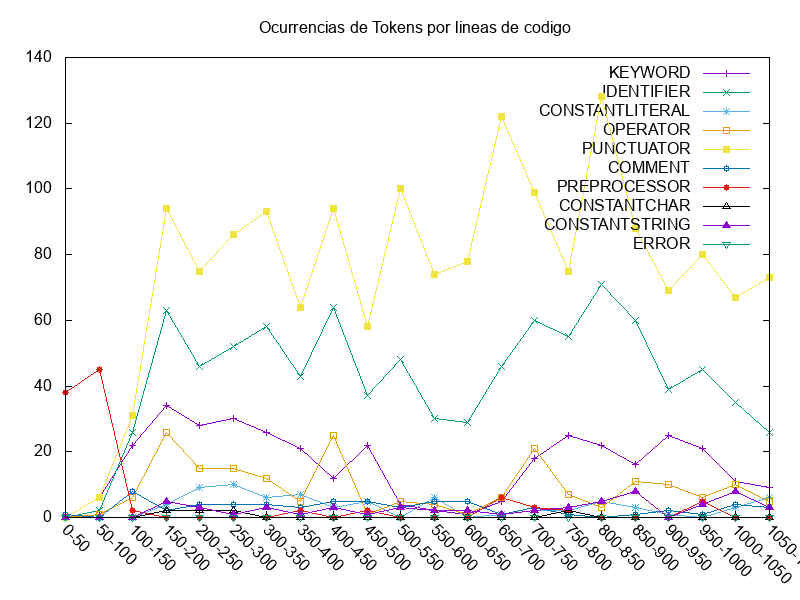
\includegraphics[scale=0.4]{histogram.png}
	\end{alertblock}
\end{frame}

\begin{frame}[fragile,allowframebreaks]{Analisis Léxico}
\begin{alertblock}{Codigo fuente}
	A continuación se presenta el codigo fuente con colores demostrando la división de Tokens.
	\end{alertblock}
\end{frame}
\begin{frame}[fragile,allowframebreaks]{Resaltado de sintaxis}~\color{MidnightBlue}\verb$# 1 "tests/1.c"$\newline\color{MidnightBlue}\verb$# 1 "<built-in>"$\newline\color{MidnightBlue}\verb$# 1 "<command-line>"$\newline\color{MidnightBlue}\verb$# 31 "<command-line>"$\newline\color{MidnightBlue}\verb$# 1 "/usr/include/stdc-predef.h" 1 3 4$\newline\newline\color{MidnightBlue}\verb$# 1 "/usr/include/stdc-predef.h" 3 4$\newline\color{Gray}\begin{verbatim}/* Copyright (C) 1991-2018 Free Software Foundation, Inc.
   This file is part of the GNU C Library.

   The GNU C Library is free software; you can redistribute it and/or
   modify it under the terms of the GNU Lesser General Public
   License as published by the Free Software Foundation; either
   version 2.1 of the License, or (at your option) any later version.

   The GNU C Library is distributed in the hope that it will be useful,
   but WITHOUT ANY WARRANTY; without even the implied warranty of
   MERCHANTABILITY or FITNESS FOR A PARTICULAR PURPOSE.  See the GNU
   Lesser General Public License for more details.

   You should have received a copy of the GNU Lesser General Public
   License along with the GNU C Library; if not, see
   <http://www.gnu.org/licenses/>.  */\end{verbatim}\leavevmode\newline\newline\newline\newline\newline\color{Gray}\begin{verbatim}/* This header is separate from features.h so that the compiler can
   include it implicitly at the start of every compilation.  It must
   not itself include <features.h> or any other header that includes
   <features.h> because the implicit include comes before any feature
   test macros that may be defined in a source file before it first
   explicitly includes a system header.  GCC knows the name of this
   header in order to preinclude it.  */\end{verbatim}\leavevmode\newline\newline\color{Gray}\begin{verbatim}/* glibc's intent is to support the IEC 559 math functionality, real
   and complex.  If the GCC (4.9 and later) predefined macros
   specifying compiler intent are available, use them to determine
   whether the overall intent is to support these features; otherwise,
   presume an older compiler has intent to support these features and
   define these macros by default.  */\end{verbatim}\leavevmode\newline\color{MidnightBlue}\verb$# 52 "/usr/include/stdc-predef.h" 3 4$\newline\color{Gray}\begin{verbatim}/* wchar_t uses Unicode 10.0.0.  Version 10.0 of the Unicode Standard is
   synchronized with ISO/IEC 10646:2017, fifth edition, plus
   the following additions from Amendment 1 to the fifth edition:
   - 56 emoji characters
   - 285 hentaigana
   - 3 additional Zanabazar Square characters */\end{verbatim}\leavevmode\newline\newline\newline\color{Gray}\begin{verbatim}/* We do not support C11 <threads.h>.  */\end{verbatim}\leavevmode\newline\color{MidnightBlue}\verb$# 32 "<command-line>" 2$\newline\color{MidnightBlue}\verb$# 1 "tests/1.c"$\newline\newline\color{MidnightBlue}\verb$# 1 "tests/1.c"$\newline\color{BlueViolet}\verb$main$\color{OliveGreen}\verb$($\color{OliveGreen}\verb$)$ \color{OliveGreen}\verb${$\newline    \color{Sepia}\verb$int$ \color{BlueViolet}\verb$a$\color{OliveGreen}\verb$;$\newline\color{OliveGreen}\verb$}$\newline
\end{frame}



{\setbeamercolor{palette primary}{fg=black, bg=yellow}
\begin{frame}[standout]
  ¿Preguntas?
\end{frame}
}


\end{document}
